\documentclass[a4paper]{report}
\usepackage{amsmath,commath,amsfonts,mathrsfs,textcomp}
\usepackage{psfrag}
\usepackage[dvips]{graphicx}
\usepackage{subfig}
\usepackage{float}
\usepackage{pdfpages}
\usepackage{pgfplots}
\usepackage{datetime}
\usepackage{rotating}
\usepackage{framed}
\usepackage{lipsum}
\usepackage{caption} 
\captionsetup[table]{skip=5pt}

\usepackage[colorlinks,
linkcolor=blue,
urlcolor=black,
anchorcolor=red,
citecolor=red]{hyperref}

%% turn on to use the Palatino font
%\usepackage[sc]{mathpazo}

%% choose the way of numbering the equations
%\numberwithin{equation}{section}                  % number the equation like (1.1.1) (1.1.2) instead of (1) (2) (3)
\renewcommand{\theequation}{\arabic{equation}}   % number the equation like (1) (2) (3) instead of (1.1.1) (1.1.2)

%% Allows customization of titles
\usepackage{titlesec} 
%\renewcommand\thesection{\Roman{chapter}} % Roman numerals for the sections
%\renewcommand\thesection{\Roman{section}} % Roman numerals for the sections
%\renewcommand\thesubsection{\Roman{subsection}} % Roman numerals for subsections
\titleformat{\chapter}[block]{\huge\bfseries\scshape}{\thechapter.}{1em}{} % Change the look of the section titles
\titleformat{\section}[block]{\Large\bfseries\scshape}{\thesection}{1em}{}
\titleformat{\subsection}[block]{\large\bfseries\scshape}{\thesubsection}{1em}{} % Change the look of the section titles

%% chapter start from the same page
%\usepackage{etoolbox}
%\makeatletter
%\patchcmd{\chapter}{\if@openright\cleardoublepage\else\clearpage\fi}{}{}{}
%\makeatother

%% the geometry of all pages
\usepackage[hmarginratio=1:1,top=35mm,bottom=35mm,left=30mm,columnsep=30pt]{geometry}

\usepackage{color}
\definecolor{shadecolor}{rgb}{0.92,0.92,0.92}

%% for boxed equations
\usepackage[skins,theorems]{tcolorbox}
\tcbset{highlight math style={enhanced,
		colframe=red,colback=white,arc=0pt,boxrule=1pt}}

%% set paragraph skip and the empty distance between two paragraphs
\setlength{\parskip}{0.4cm}
\setlength{\parindent}{0cm}

%% (I forget the function of this)
%\usepackage{xcolor}
%\makeatletter
%\def\mathcolor#1#{\@mathcolor{#1}}
%\def\@mathcolor#1#2#3{%
%	\protect\leavevmode
%	\begingroup
%	\color#1{#2}#3%
%	\endgroup
%}
%\makeatother

%% define the color of chaptername, sectionname and so on
\usepackage{sectsty}% http://ctan.org/pkg/sectsty
%\chapterfont{\color{red}}
%\sectionfont{\color{blue}}
%\subsectionfont{\color{green!80!black}}
%\subsubsectionfont{\color{purple}}
%\paragraphfont{\color{orange}}

%% fancy page head and page foot
\usepackage{fancyhdr}
\renewcommand{\sectionmark}[1]{\markright{\thesection~ ~#1}}
\renewcommand{\chaptermark}[1]{\markboth{\chaptername~\thechapter~~ #1}{}}
\fancypagestyle{IHA-fancy-style}{%
	\fancyhf{}
	\fancyhead[LE,RO]{\slshape \nouppercase{\rightmark}}
	\fancyhead[LO,RE]{\slshape \nouppercase{\leftmark}}
	\fancyfoot[C]{\thepage\ of \pageref{TheLastPage}}% Custom footer
	\renewcommand{\headrulewidth}{0.3pt}% Line at the header visible
	\renewcommand{\footrulewidth}{0.2pt}% Line at the footer visible
}
% Redefine the plain page style
\fancypagestyle{plain}{%
	\fancyhf{}%
	%	\fancyfoot[C]{\thepage\ of \pageref{LastPage}}%
	\renewcommand{\headrulewidth}{0pt}% Line at the header invisible
	\renewcommand{\footrulewidth}{0pt}% Line at the footer visible
}

%% now we can \begin a remark, definition or theorem
\newtheorem{definition}{Definition}[section]
\newtheorem{definition*}{Definition}
\newtheorem{remark}{Remark}[section]
\newtheorem{remark*}{Remark}
\newtheorem{theorem}{Theorem}[section]
\newtheorem{theorem*}{Theorem}

%% change the tilename of bib into References
\renewcommand{\bibname}{References} 

% % % % % % % % % % % % % % % % % % % % % % % % % % % % % % % % % % % % % % % % % % % % % % % % % % % % %
% % % % % % % % % % % % % % % % % % % % % % % % % % % % % % % % % % % % % % % % % % % % % % % % % % % % %
% % % % % % % % % % % % % % % % % % % % % % % % % % % % % % % % % % % % % % % % % % % % % % % % % % % % %
% % % % % % % % % % % % % % % % % % % % % % % % % % % % % % % % % % % % % % % % % % % % % % % % % % % % %
% % % % % % % % % % % % % % % % % % %        shortcuts      % % % % % % % % % % % % % % % % % % % % % % %
% % % % % % % % % % % % % % % % % % % % % % % % % % % % % % % % % % % % % % % % % % % % % % % % % % % % %
% % % % % % % % % % % % % % % % % % % % % % % % % % % % % % % % % % % % % % % % % % % % % % % % % % % % %
% % % % % % % % % % % % % % % % % % % % % % % % % % % % % % % % % % % % % % % % % % % % % % % % % % % % %
% % % % % % % % % % % % % % % % % % % % % % % % % % % % % % % % % % % % % % % % % % % % % % % % % % % % %
% % % % % % % % % % % % % % % % % % % % % % % % % % % % % % % % % % % % % % % % % % % % % % % % % % % % %

% domain and integrals
\newcommand{\intO}{\int_{\Om}}
\newcommand{\intpO}{\int_{\partial\Om}}
\newcommand{\Om}{\Omega}
\newcommand{\p}{\partial}

% half
\newcommand{\half}{\dfrac{1}{2}}

% exterior calculus
\newcommand{\ed}{\mathrm{d}}


% math bold: vector
\newcommand{\bu}{\boldsymbol{u}}
\newcommand{\tbu}{\tilde{ \boldsymbol{u} }}
\begin{document}
\pagestyle{IHA-fancy-style}
%%%%%%%%%%%%%%%%%%%%%%%%%%%%%%%%%%%%%%%%%%%%%%%%%%%%%%%%%%%%%%%%%%%%%%%%%%%%%%%%%%%%%%%%%%%%%%%%%%%%%%%%%%%%%%%%%%%%%%%%%%%%%%%%%%%%%%%%%%%%%%%%%%%%%%%%%%%%%%%%%%%%%%%%%%%%%%%%%%%%%%%%%%%%%%%%%%%%%%%%%%%%%%%%%%%%%%%%%%%%%%%%%%%%%%%%%%%%%%%%%%%%%%%%%%%%%%%%%%
\section*{Scalar Poisson}
$ h- $convergence:
\begin{figure}[h!]
	\centering{
		\subfloat{
			\begin{minipage}[t]{0.5\textwidth}
				\centering
				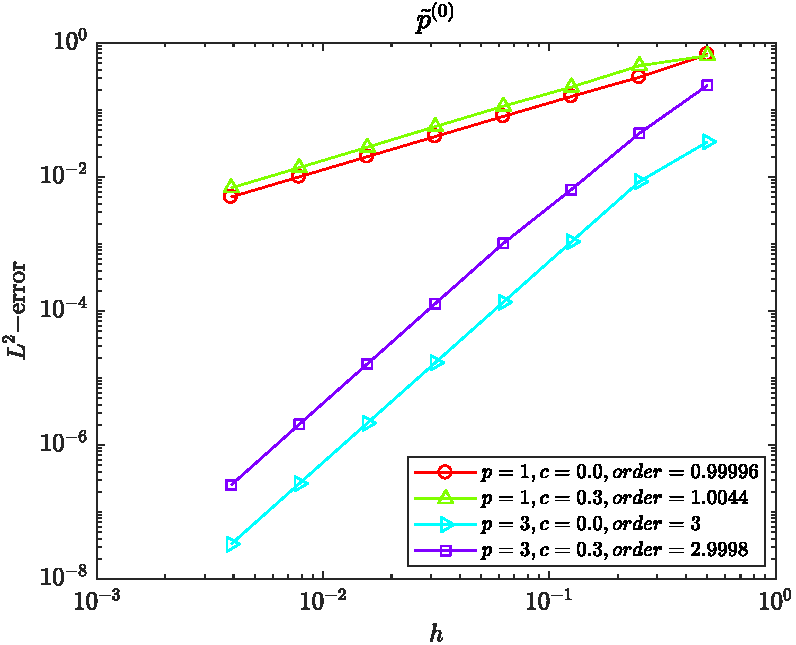
\includegraphics[width=1\linewidth]{../h_convergence/h_p0_L2}
			\end{minipage}
		}
		\subfloat{
			\begin{minipage}[t]{0.5\textwidth}
				\centering
				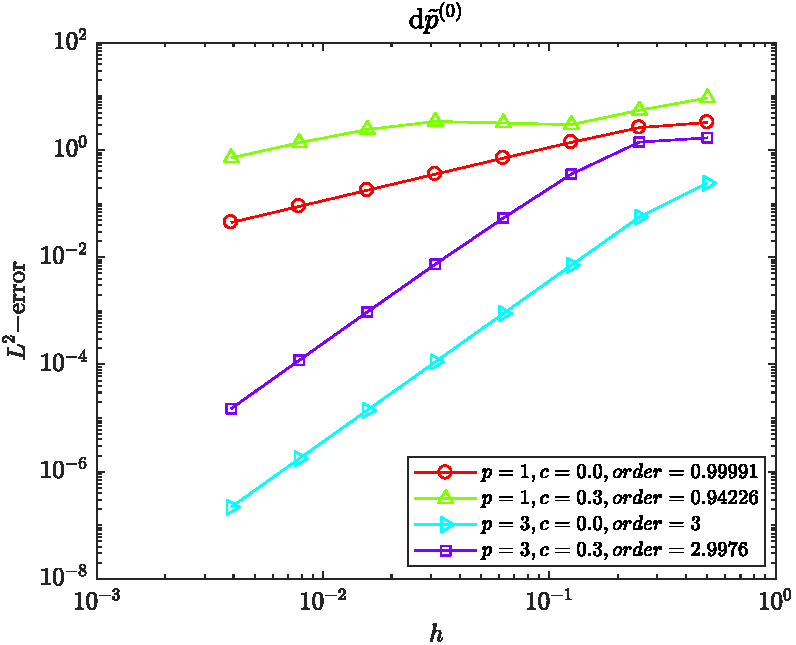
\includegraphics[width=1\linewidth]{../h_convergence/h_dp0_L2}
			\end{minipage}
		}\\
		\subfloat{
			\begin{minipage}[t]{0.5\textwidth}
				\centering
				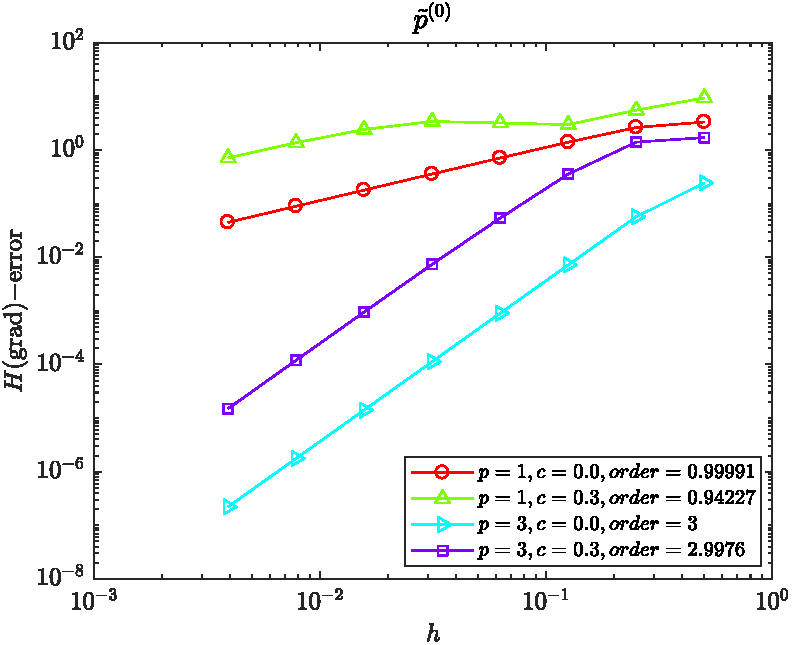
\includegraphics[width=1\linewidth]{../h_convergence/h_p0_H}
			\end{minipage}
		}
		\subfloat{
			\begin{minipage}[t]{0.5\textwidth}
				\centering
				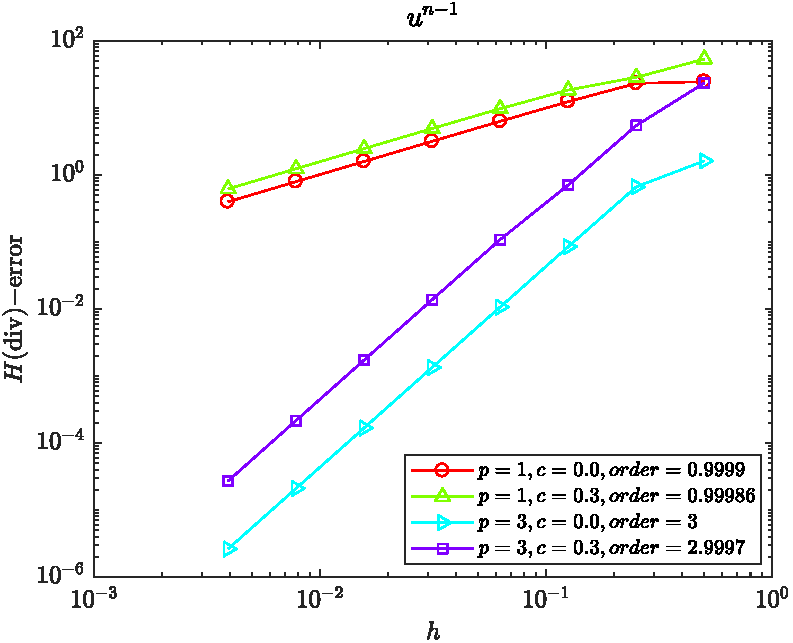
\includegraphics[width=1\linewidth]{../h_convergence/h_u_H}
			\end{minipage}
		}\\
		\subfloat{
		\begin{minipage}[t]{0.5\textwidth}
			\centering
			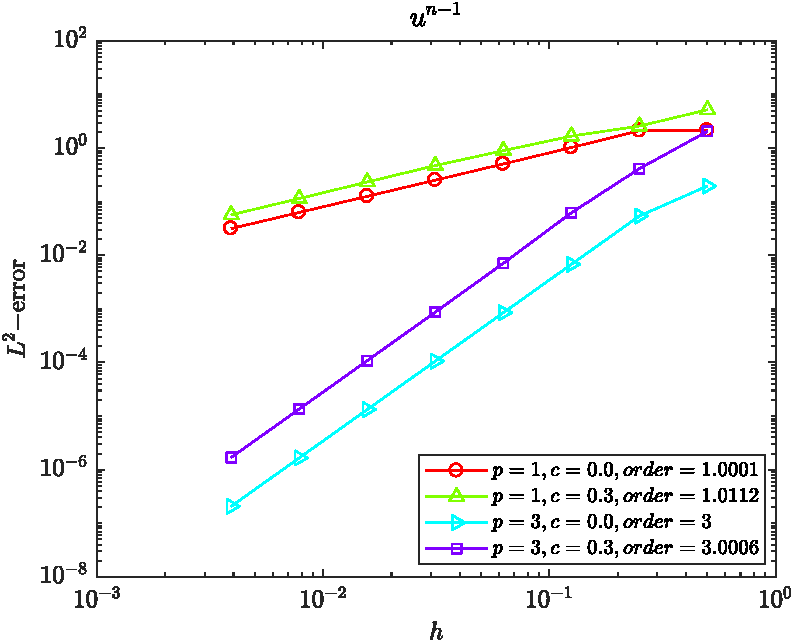
\includegraphics[width=1\linewidth]{../h_convergence/h_u_L2}
		\end{minipage}
		}
		\subfloat{
		\begin{minipage}[t]{0.5\textwidth}
			\centering
			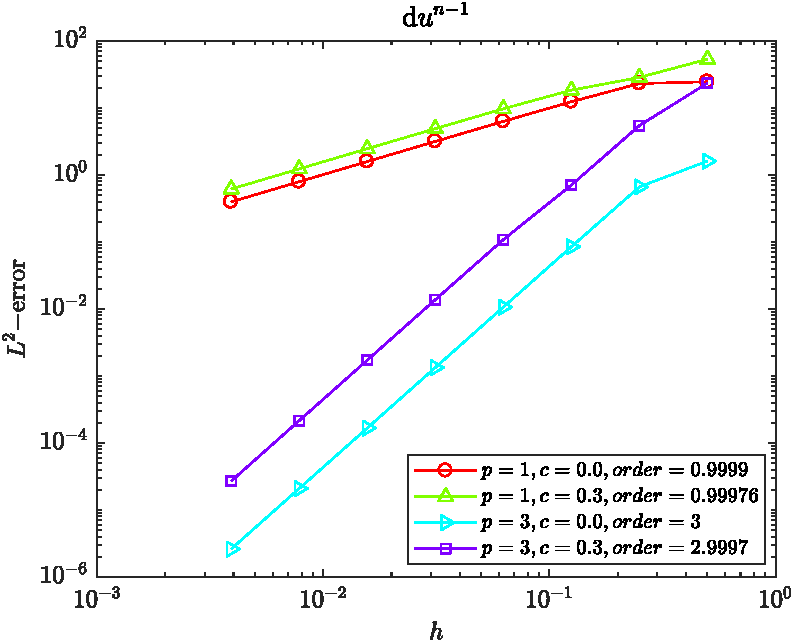
\includegraphics[width=1\linewidth]{../h_convergence/h_du_L2}
		\end{minipage}
		}
		\caption{The $ h- $convergence.}
		\label{Fig: h convergence}
	}
\end{figure}


$ p- $convergence:
\begin{figure}[h!]
	\centering{
		\subfloat{
			\begin{minipage}[t]{0.5\textwidth}
				\centering
				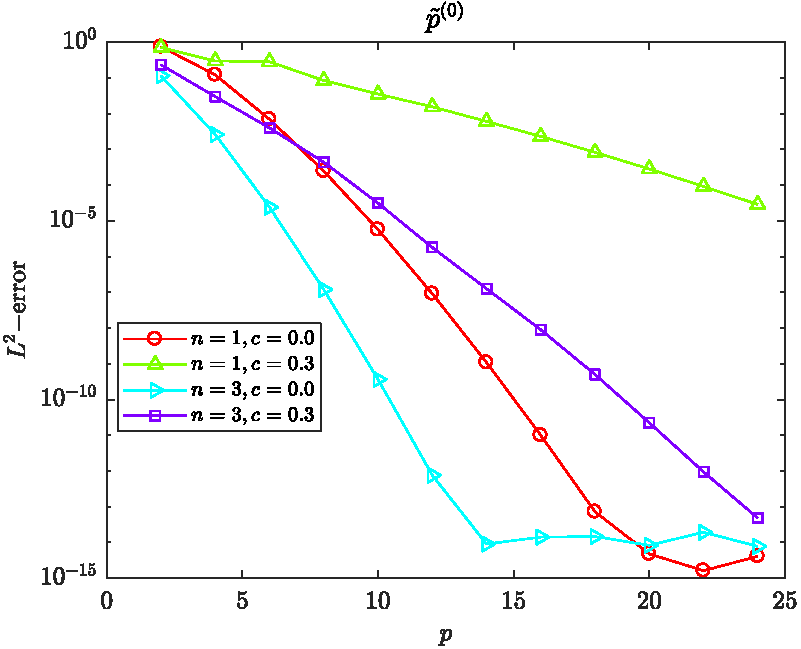
\includegraphics[width=1\linewidth]{../p_convergence/p_p0_L2}
			\end{minipage}
		}
		\subfloat{
			\begin{minipage}[t]{0.5\textwidth}
				\centering
				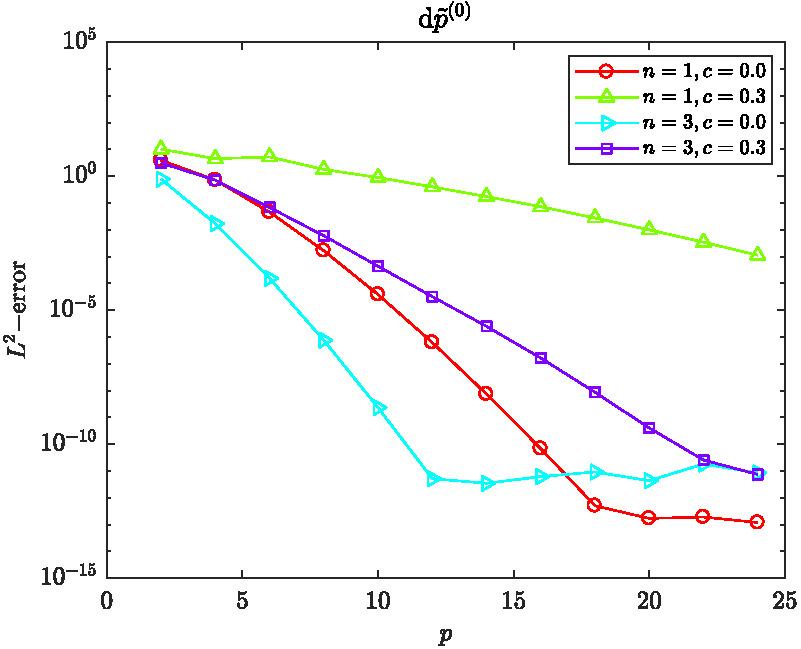
\includegraphics[width=1\linewidth]{../p_convergence/p_dp0_L2}
			\end{minipage}
		}\\
		\subfloat{
			\begin{minipage}[t]{0.5\textwidth}
				\centering
				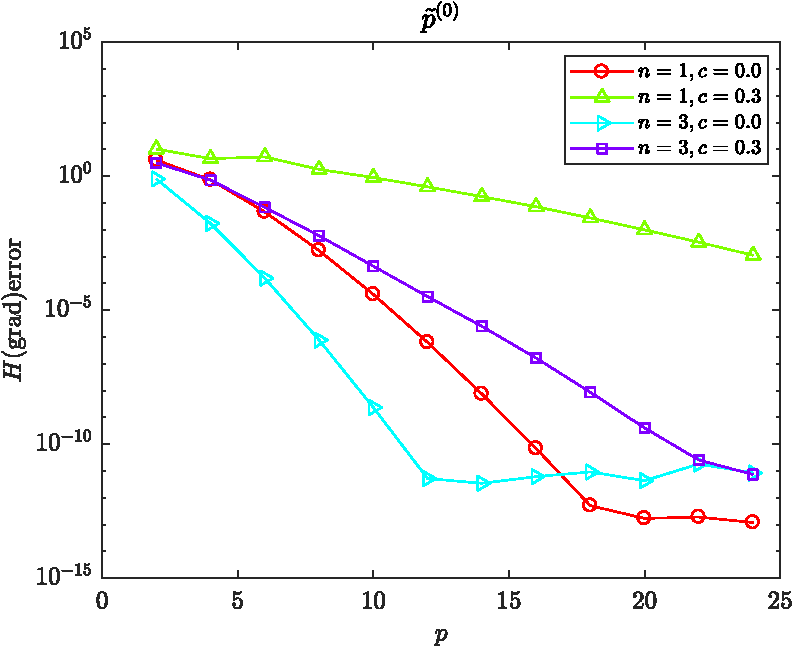
\includegraphics[width=1\linewidth]{../p_convergence/p_p0_H}
			\end{minipage}
		}
		\subfloat{
			\begin{minipage}[t]{0.5\textwidth}
				\centering
				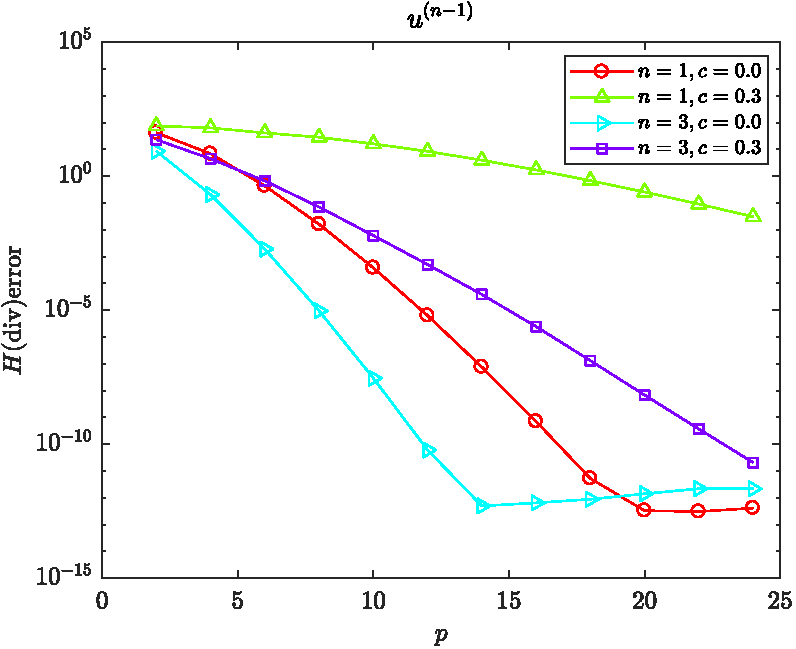
\includegraphics[width=1\linewidth]{../p_convergence/p_u_H}
			\end{minipage}
		}\\
		\subfloat{
			\begin{minipage}[t]{0.5\textwidth}
				\centering
				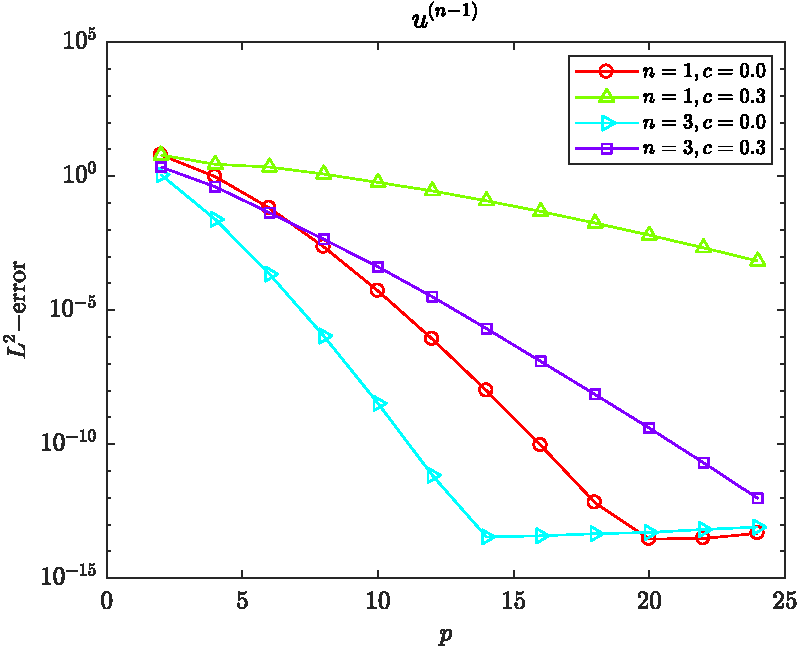
\includegraphics[width=1\linewidth]{../p_convergence/p_u_L2}
			\end{minipage}
		}
		\subfloat{
			\begin{minipage}[t]{0.5\textwidth}
				\centering
				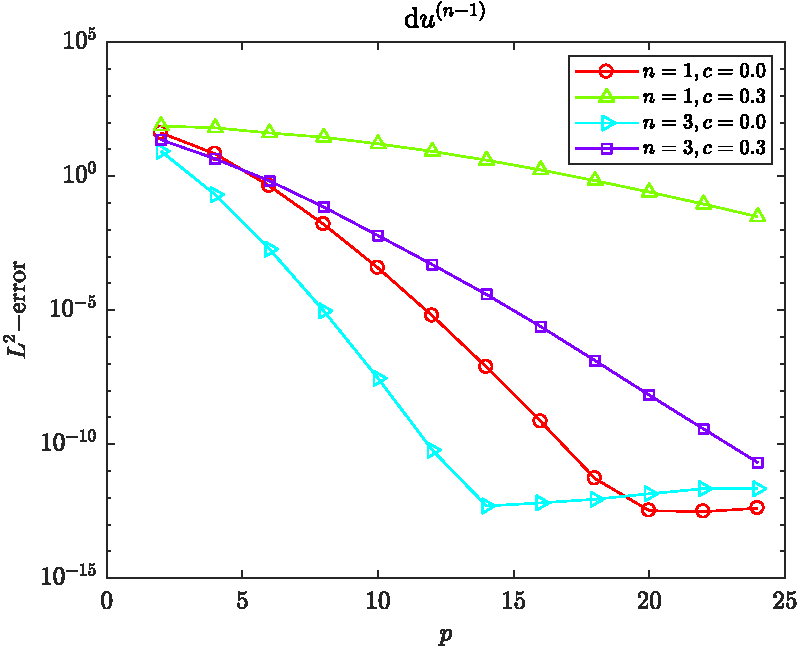
\includegraphics[width=1\linewidth]{../p_convergence/p_du_L2}
			\end{minipage}
		}
		\caption{The $ p- $convergence.}
		\label{Fig: p convergence}
	}
\end{figure}

\clearpage
Time efficiency:
\begin{figure}[h!]
	\centering
	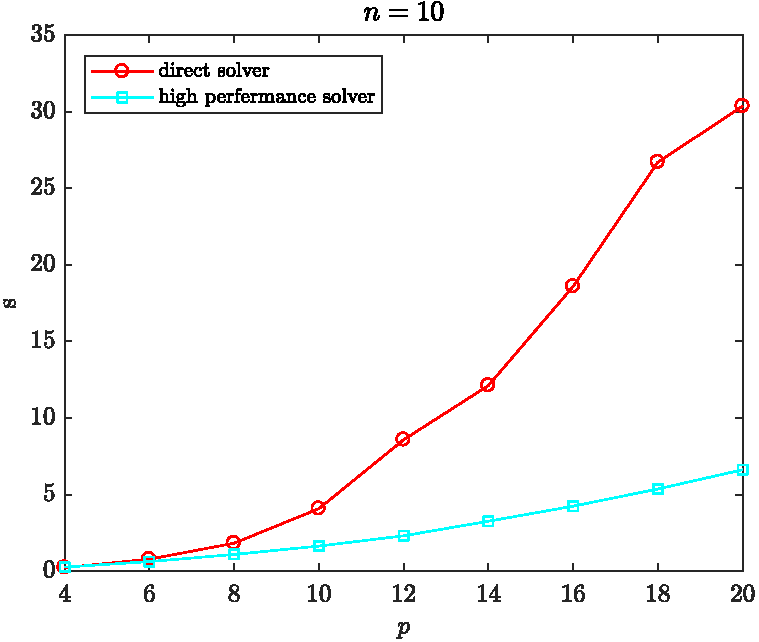
\includegraphics[width=0.7\linewidth]{../TIME_comparison/cost_comp}
	\caption{time efficiency comparison}
	\label{fig:costcomp}
\end{figure}

Condition number:
\begin{figure}[h!]
	\centering
	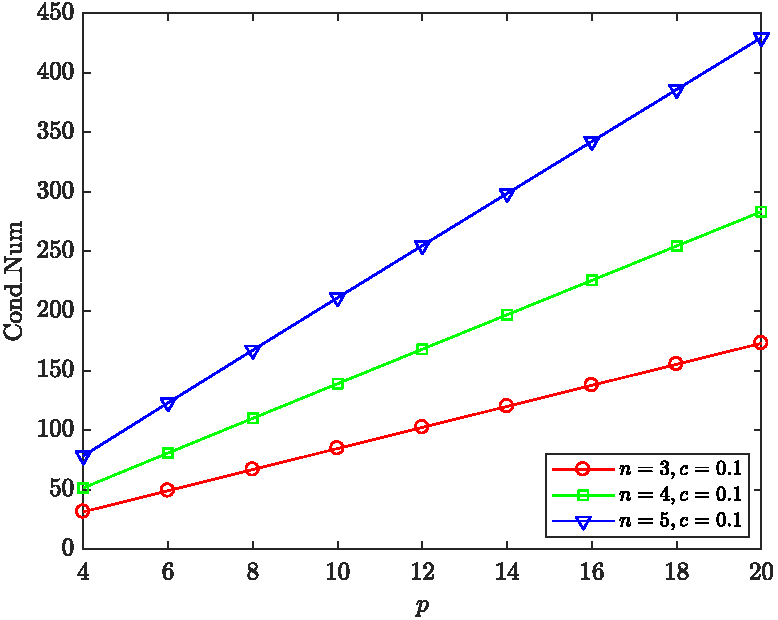
\includegraphics[width=0.7\linewidth]{../COND_NUM/COND_NUM}
	\caption{Condition number of the system for $ \phi $}
	\label{fig:condnum}
\end{figure}



%\clearpage
%\bibliographystyle{apalike}
%\bibliographystyle{abbrv}
%\addcontentsline{toc}{chapter}{References}
%\bibliography{C:/Users/yzhang24/Dropbox/Materials/library}

\label{TheLastPage}
\end{document}